\documentclass{article}
\usepackage{amsfonts}
\usepackage{amsthm}
\usepackage{amssymb}
\usepackage{amsmath}
\usepackage{graphicx}
\usepackage{subcaption}

\newcommand{\new}[1]{
    \vspace{2mm}
    \noindent
    \textbf{
    \underline{#1}}
}

\def\calO{{\mathcal{O}}}
\def\th{{\theta}}
\def\_{{\hspace{1mm}}}
\def\<{{\langle}}
\def\>{{\rangle}}


\newcounter{problemcnt}
\setcounter{problemcnt}{0}

\newcommand{\Problem}{{
    \vspace{5mm}
    \stepcounter{problemcnt}
    \noindent
    \arabic{problemcnt}. 
}
}

\newcommand{\nProblem}[1]{
    \vspace{5mm}
    \noindent
    \setcounter{problemcnt}{#1}
    \arabic{problemcnt}. 
}


\newcommand{\Proof}{{
    \vspace{2mm}
    \noindent
    \textbf{
    \underline{Proof}}
}
}

\newcommand{\textOr}{
    {
        \hspace{5mm}
        \textrm{or}
        \hspace{5mm}
    }
}

\newcommand{\textAnd}{
    {
        \hspace{5mm}
        \textrm{and}
        \hspace{5mm}
    }
}

\begin{document}
\begin{center}
\LARGE
PHYS 201 Problemset 9

\Large
Daniel Son
\end{center}

\normalsize

\nProblem{1}
Find the electromotive force induced 
on a square wire when the wire is passing 
through the center. 

\begin{center}
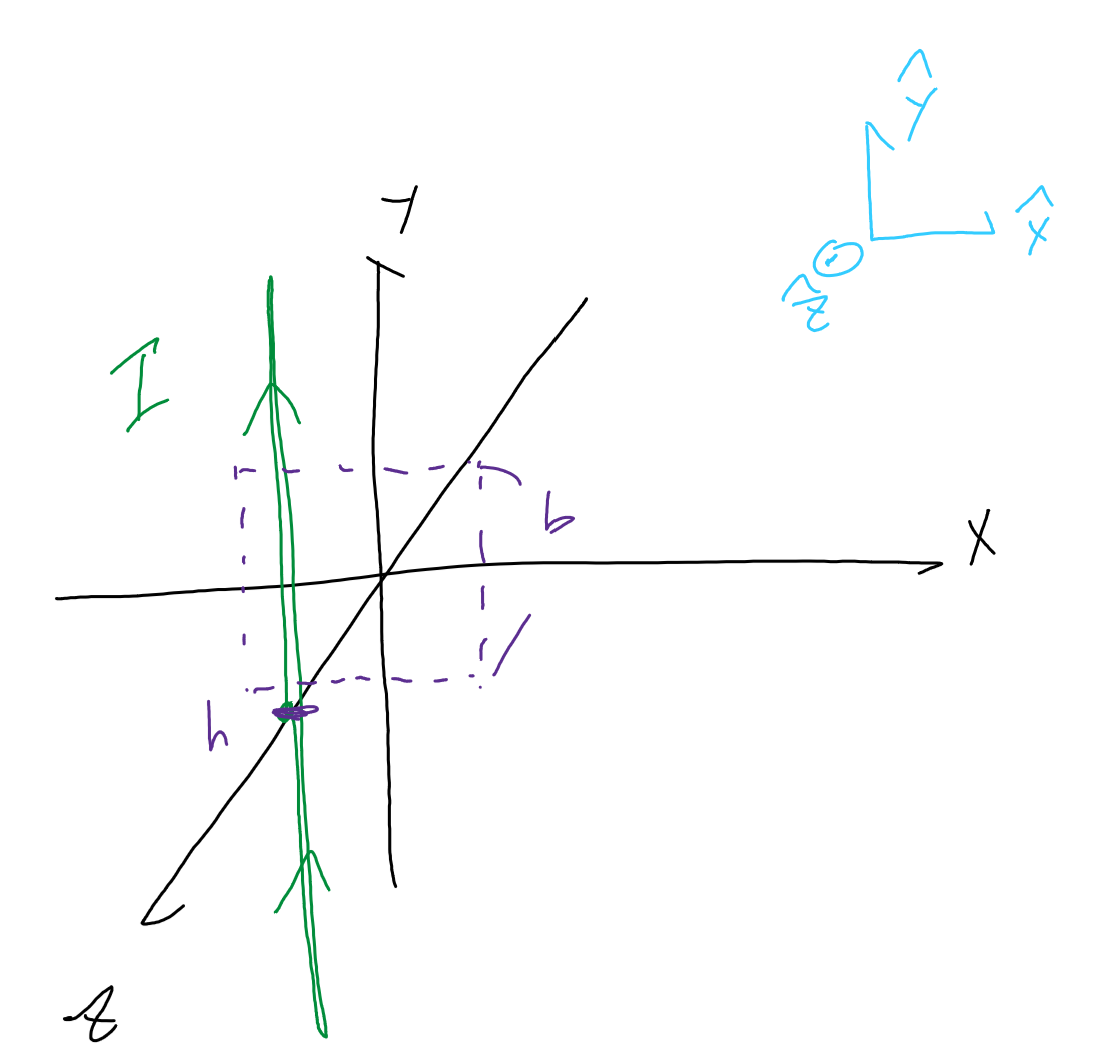
\includegraphics[width = .5\linewidth]{Q1_setup.png}

Figure 1: setup
\end{center}

To begin with, we determine the magnetic force 
along the xy-plane. Notice that by symmetry, 
the magnetic field is independent of the y 
axis. Thus, fix $y = z = 0$. We want to 
derive an equation for $\vec{B}(x)$. 

Recall:
\[
    B = 
    \frac{\mu_0I}
    {2\pi r}
\]
And that the direction of $B$ is determined 
by the right hand rule. We write:

\[
    \vec{B}(x) = 
    \frac{\mu_0 I}
    {2\pi \sqrt{x^2+h^2}}
    -\overline{{\<h, 0, x\>}}
\]

Where the bar denotes the unit vector. 
As to understand how the directional vetor is derived 
refer to the following figure:

\begin{center}
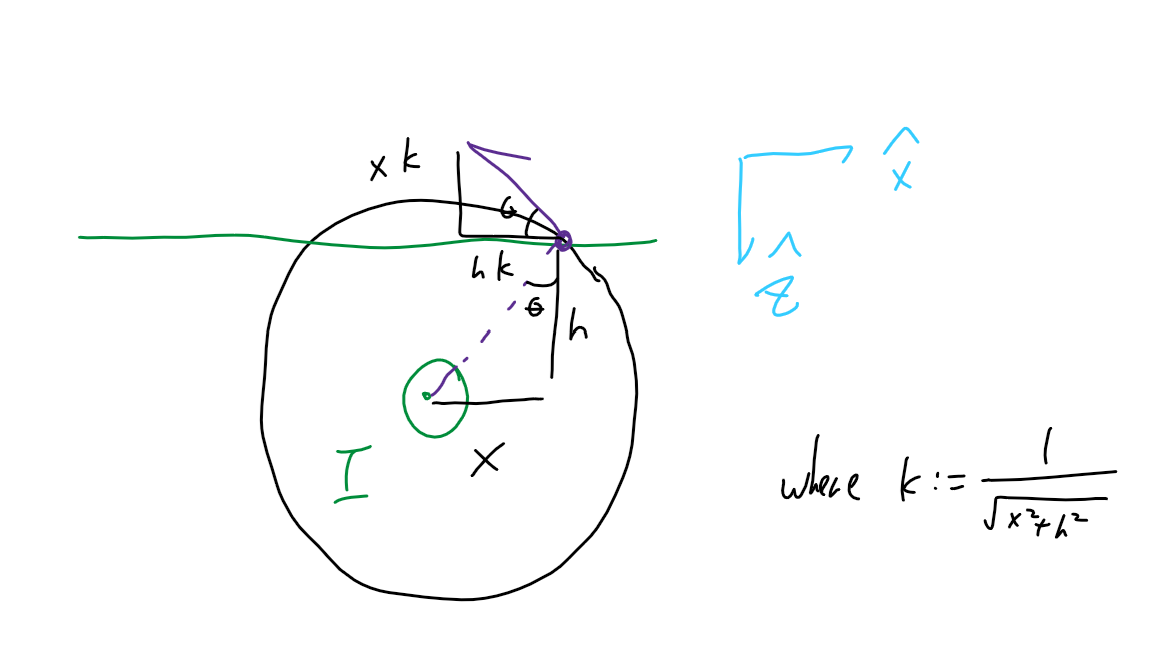
\includegraphics[width = .5\linewidth]{Q1_cut.png}

Figure 2: horizontal cut
\end{center}

Moreover, note that:

\[
    \vec{B}\cdot \vec{z} 
    = 
    \frac{\mu_0 I}
    {2\pi (x^2+h^2)}
    (-x)
\]

Now, compute the electromotive force 
by Faraday's Law. Write:

\def\EMF{{\mathcal{E}}}

\[
    \left.
    \EMF = 
    -
    \frac{d\Phi} {dt}
    \right|
    _{x = 0}    
\]

We can compute:
\[
    \left.
        \frac{d}{dx}
        \oint_{\gamma}
        \vec{B}d{\vec{a}}
    \right|_{x = 0}
    =
    b(\vec{B}\cdot\vec{z}
    \bigg|_{x = b/2}
    -\vec{B}\cdot\vec{z}
    \bigg|_{x = -b/2}
    )
\]

As we have established earlier, we write:
\[
    = b 
    \frac{\mu_0 I}
    {2 \pi (b^2/4+h^2)}
    \left[    
        -\frac{b}{2}
        -\frac{b}{2}
    \right]
    =
    -b^2
    \frac{\mu_0 I}
    {2 \pi (b^2/4+h^2)}
\]

By the chain rule:


\[
    \boxed{
    \left.
    \EMF = 
    -
    \frac{d\Phi} {dt}
    \right|
    _{x = 0}   
    =
    -
    \frac{dx}{dt}
    \left.
    \frac{d\Phi} {dx}
    \right|
    _{x = 0} 
    =
    \frac{2vb^2\mu_0I}{\pi(b^2+4h^2)}
    }
\]

\qed


\newpage

\nProblem{2}
A rod connected to a circuit 
is passing through a uniform magnetic 
field. Answer the following problems:
\begin{enumerate}
    \item When does the rod stop?
    \item How much has the rod traveled?
    \item What can be said about the energy of the system?
\end{enumerate}

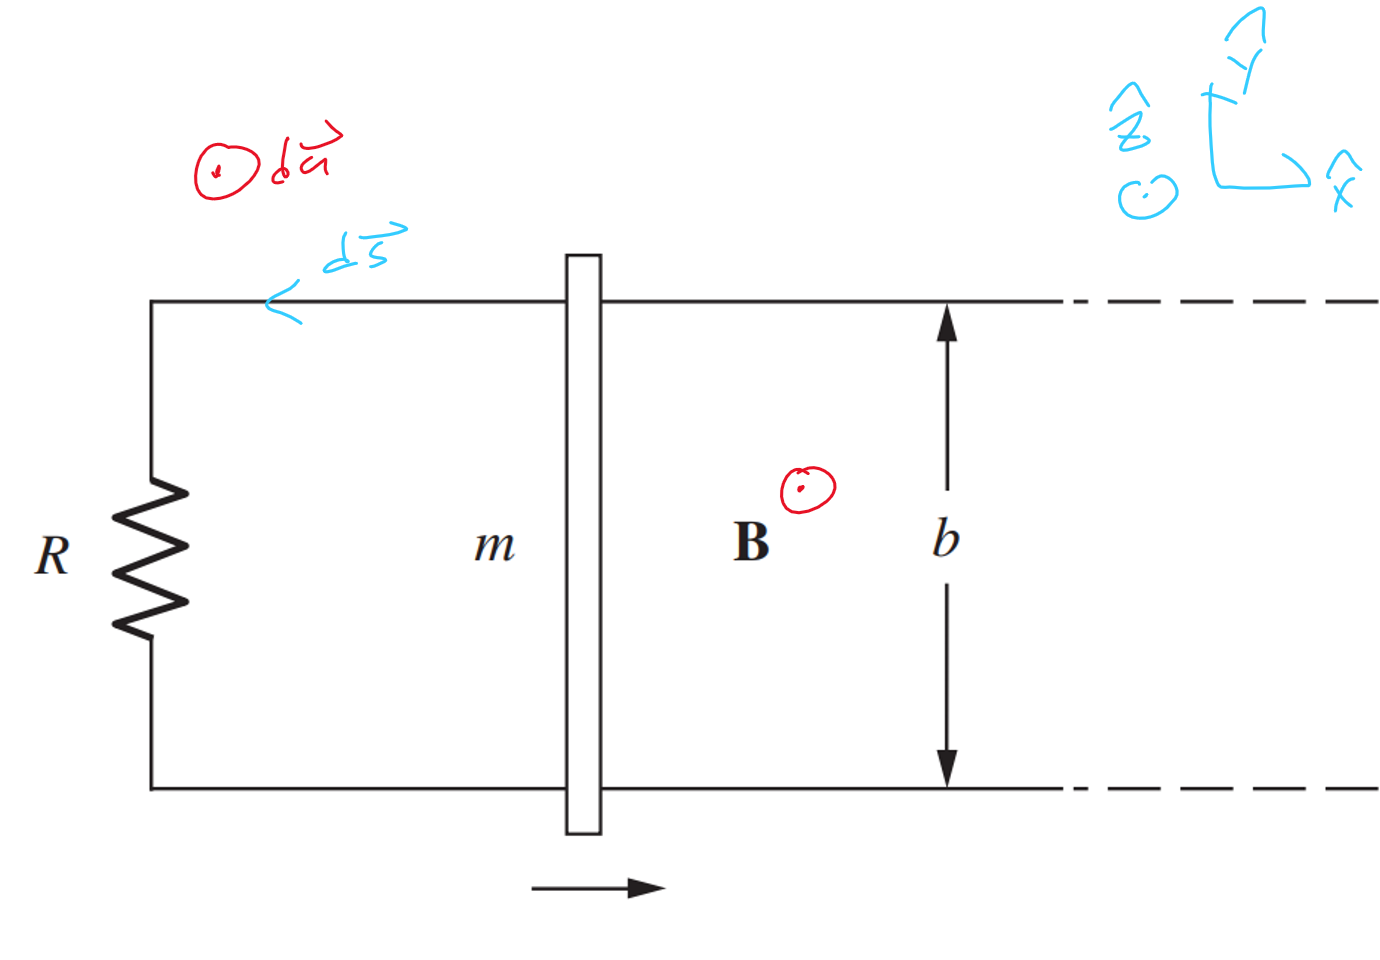
\includegraphics[width = .7\linewidth]{Q2_setup.png}

\new{Solution}
It seems reasonable to first come up 
with a time dependent equation of
the vertical velocity of the rod. Let 
$v(t)$ be a scalar function that describes 
the x direction velocity. Denote the initial 
velocity as $v_0$. 

We want to compute the current induced 
on the rod. The induced current 
will be perpendicular to the direction of 
the magnetic field. This in turn will 
create a Lorentz force that is opposite 
of the direction of movement. 

Define the direction of the surface vector 
$d\vec{a}$ to point out of the surface. 
Also, let $d\vec{s}$ to be counterclockwise. 

Now that all the directions are established 
move on to compute the integrals. To 
invoke Faraday's law, compute the magnetic 
flux. Write:

\[
    \Phi = \oint_{loop} \vec{B}d\vec{a}
     = lbB
\]

Where l denotes the horizontal distance 
from the resistor to the rod. 

By Faraday:

\[
    \EMF = 
    -\frac{d\Phi}{dt}
     = -vbB
\]
This derivative is justified by observing 
that the time derivative of $l$ is $v$. 

Apply Ohm's law to compute the current. 

\[
    \EMF = I R
\]
\[
    I = -\frac{vbB}{R}
\]

The current flows clockwise. 
Applying the right hand rule, 
we deduce that the magnetic field 
is towards the $-x$ direction. 

To compute the magnitude of the 
force exerted on the rod, consider
the following equation:

\[
    qv_{drift} = Ib
\]

where $q$ is the total moving charge 
inside the rod. 

Assuming that there is no electric field, 
we write:
\[
    F = qv_{drift}B
\]

We consider only the magnitudes, and 
$v_{drift}$, $B$ are perpendicular. Thus 
the equation is justified. Ignore self 
inductance. Also, $F = ma$. We write:

\[
    ma = -IbB = -\frac{vb^2B^2}{R}
\]
\[
    a = -\frac{vb^2B^2}{mR}
\]
\[
    \frac{dv}{dt} \cdot \frac{1}{v}
     = 
     -\frac{b^2B^2}{mR}
\]

Noticd that the left side is the logarithmic derivative. 
Write:

\[
    ln(v) = \frac{-b^2B^2}{mR}t+C 
\]


The initial condition $v(0) = v_0$ must be met. We conclude:
\[
    v = v_0\textrm{Exp}\left[
-\frac{b^2B^2}{mR}t
    \right]
\]

To answer the first question, the rod theoretically never stops. 
As for the distance traveled we take the integral:

\[
    \int_{t = 0}^{\infty} v_0\textrm{Exp}\left[
-\frac{b^2B^2}{mR}t
    \right]
    = 
    \left.
        -
        \frac{v_0mR}
        {b^2B^2}
        \textrm{Exp}\left[
-\frac{b^2B^2}{mR}t
    \right]
    \right|_{t = 0}^{{\infty}}
     = 
     \boxed{
     \frac{v_0mR}{b^2B^2}
     }
\]

The total kinetic energy lost is:
\[
    \Delta K = 
    \frac{1}{2} mv_0^2
\]

The magnetic field has done no work. Nonetheless, 
energy is dissipated through the resistor. Recall
$P = VI$ and we integrate the power over time to 
measure the energy lost through the resistor. Write:

\[
    \Delta E = \int_{t = 0}^{\infty} Pdt = 
    \int_{t = 0}^{\infty} I^2Rdt 
\]

Recall the relationship between the current and 
the rod speed:

\[
    I = -\frac{vbB}{R}
    =
    -\frac{v_0bB}{R}\textrm{Exp}\left[
-\frac{b^2B^2}{mR}t
    \right]
\]

Thus:

\[
    \Delta E =  \int_{t = 0}^{\infty}
    \left(
    -\frac{v_0bB}{R}\textrm{Exp}\left[
-\frac{b^2B^2}{mR}t
\right]
\right)^2Rdt
= \int_{t = 0}^{\infty}
    \frac{v_0^2b^2B^2}{R}\textrm{Exp}\left[
-\frac{2b^2B^2}{mR}t
\right]
dt
\]

\[
    =-\frac{mv_0^2}{2}\textrm{Exp}
    \left[
        -\frac{-2b^2B^2}{mR}t
    \right] 
    \bigg|^\infty_0
     = \frac{1}{2}mv_0^2
\]
And hence, $\Delta E = \Delta K$ as desired. 

\qed

\Problem
A ring-shaped wire of radius r is placed in a solenoid of 
infinite length. The current through the solenoid is given 
as a function of time as $I(t)=I_0cos(\omega t)$. The solenoid 
has a radius of $b$ and has $n$ turns per unit. Answer the following 
questions. 
\begin{itemize}
    \item What is the current through the wire?
    \item For what values does the magnetic force reach maximum?
    \item How does the magnetic force affect the wire?   
\end{itemize}

\new{Solution}
Recall the formula for magnetic force inside the solenoid. 
The field is uniform and the magnitude is given by:

\[
    \vec{B} = \mu_0nI(t)
\]

Also, by the right hand rule, the magnetic field points upwards. 

Define the positive current direction to be counterclockwise. Also 
denote the induced current as $I_r$ and the solenoid current as 
$I$. 

\[
    \EMF = \frac{d\Phi}{dt}
    =
    -\mu_0 n r^2 \pi \frac{dI}{dt}
    = 
 \mu_0 n r^2 \pi \omega I_0 sin(\omega t)
\]

By Ohm's law:

\[
    I_rR = 
 \mu_0 n r^2 \pi \omega I_0 sin(\omega t)
\]

So, 
\[
    \boxed {
    I_r = \frac{ \mu_0 n r^2 \pi \omega I_0 sin(\omega t)}{R}
    }
\]

Move on to compute the magnitude of magnetic force. Assume 
$\vec{E} = 0$. By the Lorentz force law:

\[
    \vec{F} = q\vec{v} \times \vec{B}
\]

We observe that $q\vec{v}$ is parallel to $I_r$ and $B$ is 
perpendicular to $I$. In terms of magnitude:

\[
    \vec{F} = CI_r\vec{B}
\]

Moreover, the magnetic field is a constant multiple of $I$. 
We write:
\[
    \vec{F} = CI_rI
\]
Where $C$ is a constant independent of time. Combining previous results, 
we again simplify:

\[
    \vec{F} = Csin(\omega t) cos(\omega t)
    = Csin(\omega 2t)
\]

Thus, $\vec{F}$ achieves maximum magnitude when $2t = (n+1/2)\pi$ 
or 

\[
    \boxed{
    t = (2n+1)\pi/4 \hspace{5mm}\textrm{where}\hspace{5mm} n = (0, 1, 2, \dots)
    }
    \]

Finally, consider the direction of the magnetic force. 
$q\vec{b} \parallel I$ and applying the right hand rule on 
$I$ and $B$ shows that the magnetic force directs radially outwards. 
Hence, depending when the force is measured, the magnetic force 
might strech or shrink the wire. However, the vertical force will 
always be zero. 

\qed

\Problem
A rectangular wire is moving away from an infinite wire with current 
100A. Compute the electromotive force on the wire when the loop 
is 15 cm away from the wire. How large must the resistance of the wire 
be in order that self inductance can be ignored? The dimensions of 
the rectangular wire is of width 10cm and length 15cm. The loop is moving 
away in a speed of 5m/s. 

\new{Solution}
First, ignore self inductance. By Faraday's law, it suffices 
to compute the change of magnetic flux through the wire. 
We compute the change of flux depending on the displacement from 
the wire (say x). Then, apply the chain rule to compute EMF. 

Define the x-direction to be the direction where the loop is moving. 
Also, let the suface vector to point upwards. 
Write:

\[
    \frac{d \Phi}{dx} = w(-B_{r = x}+B_{r = x+l})
\]

where $w = 8cm$, $l = 10cm$. Moving on, recall the formula for 
the magnitude of the magnetic field induced by a straight wire:

\[
    B = \frac{\mu_0 I}{2\pi r}
\]

\newpage
Thus, 

\[
    \frac{d \Phi}{dx} = w\left(-\frac{\mu_0I}{2\pi x}+
    \frac {\mu_0 I} {2\pi (x+l)}\right)
    = 
    w
    \frac{\mu_0 I}{2\pi}
    \left(
        \frac{1}{x+l} - \frac{1}{x}
    \right)
    = 
w
    \frac{\mu_0 I}{2\pi}
    \left(
        \frac{l}{x(x+l)}
    \right)
\]


By Faraday:

\[
    \EMF = 
    -\frac{d\Phi}{dt} 
    = -\frac{d\Phi}{dx} \frac{dx}{dt}
    =-wv
    \frac{\mu_0 I}{2\pi}
    \left(
        \frac{l}{x(x+l)}
    \right)
    -\approxeq 2.1\cdot 10^{-5} V
\]

The flux is decreasing in magnitude, but the signs are negative. 
Hence, absolute flux increases. The EMF has an opposite sign. 
$d\vec{s}$ is counterclockwise, so the current is clockwise. 

Now, move on to compute the resistance which makes self inductance 
ignorable. Let $\Phi$ denote the magnetic flux induced by the wire, 
and $\Phi_l$ the self-induced magnetic flux. We can rigorously 
compute $\Phi_l$ by Biot-Savat's law, but we use a dummy estimate. 

Assume magnetic field inside the loop to be uniformly:
\[
    B_l = \frac{\mu_0I_l}{2\pi d}
\]

where $I_l$ is the loop current, and $d$ is a characteristic radius, 
say $d = 4cm$. Computing the change of the flux:

\[
    \frac{d\Phi_l}{dt} = -\frac{dB_l}{dt}(lw) =
    \approxeq 
    \frac{\mu_0 I_l w l}{2\pi d} \frac {v}{h}
    \]

Where $h$ is the mean distance from the wire to the loop. 
$h \approxeq 20cm$. 
We wish that the self-induced EMF is smaller compared to 
the wire-induced EMF. Write:

\[
    |\frac{d\Phi}{dt}| \gg |\frac{d\Phi_l}{dt}|
\]

\[
    wv
    \frac{\mu_0 I}{2\pi}
    \left(
        \frac{l}{x(x+l)}
    \right)
    \gg
   \frac{\mu_0 I_l w l}{2\pi d} \frac {v}{h}
\]
By cancellation, we write:
\[
    \frac{I}{x(x+l)} \gg \frac{I_l}{dh} = \frac{\EMF / R}{dh}
\]
We want:
\[
    R \gg \frac{\EMF x (x+l)}{Idh}
\]
Through a rough computation, we realize that the left hand 
side is in the order of $10^{-7}\Omega$. It is reasonable 
to assume that the loop has much larger resistance than 
this value. \qed.  

\Problem

Estimate the inductance of a solenoid with a length of 
2m and a diameter of 10cm. The solenoid is single layered, and 
has 1200 turns. What is the approximate error?

\new{Solution}

Recall the definition of inductance:
\[
    L := \Phi / I
\]
Where $\Phi$ is the magnetic field, and $I$ is the current 
through the solenoid. The linear dependance between the flux 
and the current is implied by the Biot-Savat law. This motivates 
the definition of inductance. 

Ignore edge effects. The magnetic field is uniformly:
\[
    B = \mu_0 n I
\]
where n is the density of the turns. Multiply the magnetic 
field magnitude by the total area created by the solenoid loop. 
\[
    \Phi = \mu_0 n I (2\pi r^2) N = 
    \frac{\mu_0 N^2 I (2\pi r^2)}{l}
\]
where $r$ is the radius. 

Applying the definition of inductance, again write:

\[
    \boxed{
    L =    \frac{\mu_0 N^2 (2\pi r^2)}{l}
    \approxeq 7.11\cdot 10^{-3}T/A \textrm{ or } H
    }
\]

The wider the radius, the shorter the length of the solenoid, 
the error will be greater. The magnetic flux is overestimated 
in our idealized example. Simply assume the error to be in the order 
or radius divided by the length. This is:
\[
    \epsilon = 10cm/2m = 5\%
\]


\Problem
A circuit is presented below. The switch is remained closed 
for a few seconds. At $t = 0$, the switch is opened. Plot 
the voltage at point A, B as a function of time. 
\begin{center}
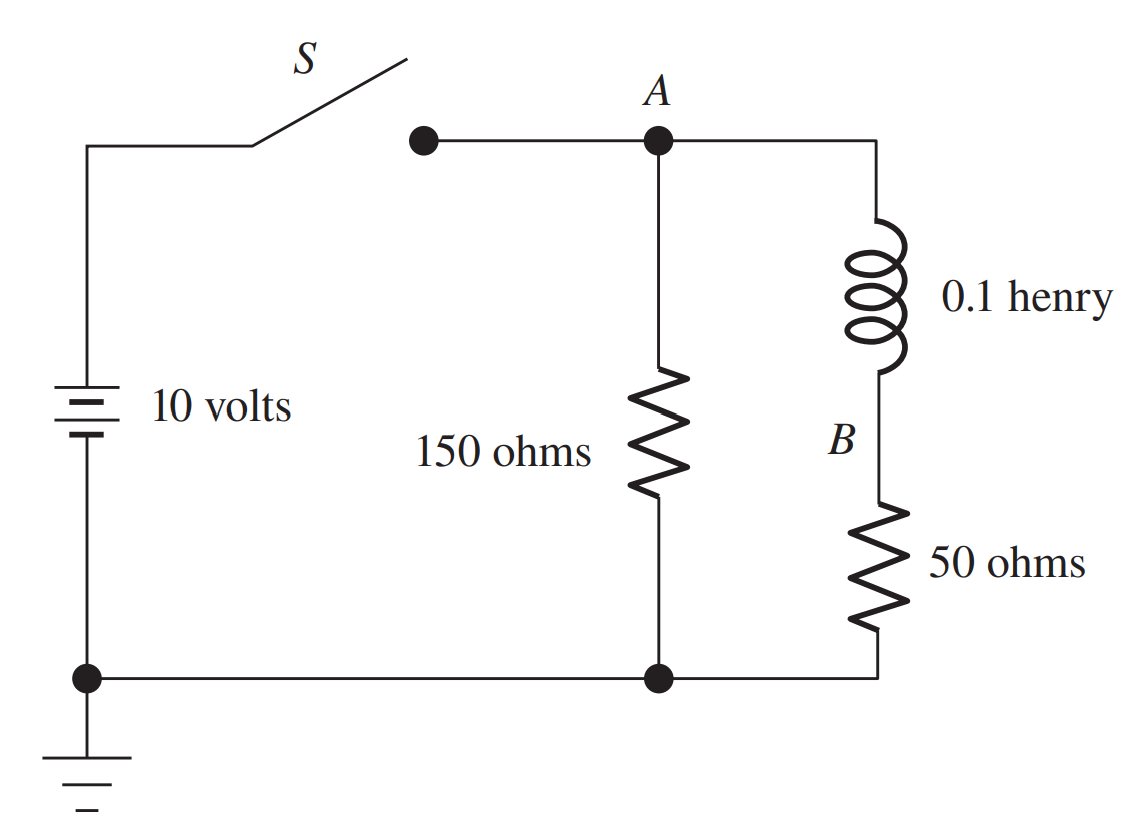
\includegraphics[width = .5\linewidth]{Q6_setup.png}
\end{center}

\new{Solution}
Here is the plot:
\begin{center}
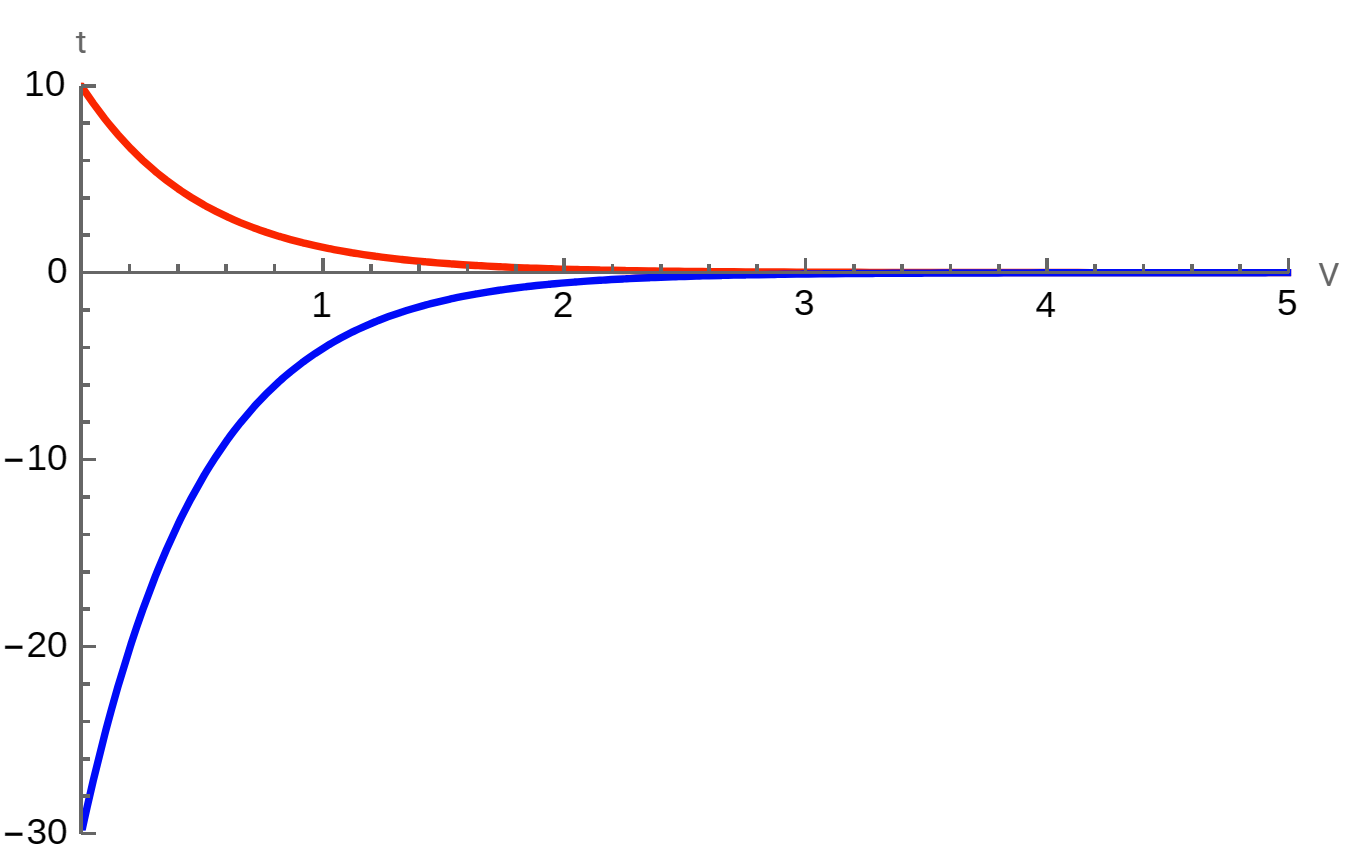
\includegraphics[width = .5\linewidth]{Q6_plot.png}
\end{center}

And here comes the reasoning. 
A few seconds is enough to bring the current to an 
equilibrium state. Thus, the solenoid can be ignored. 
It becomes trivial to observe, that at time $t = 0$, 
$V_A = V_B = 0$. By Ohm's law, compute the current 
through the solenoid at equilibrium. 

\[
    V_0 = I_0\cdot R_{eff} \textAnd
    I_0 = 15V/50\Omega = .2A
\]

Now, we consider the current after the switch has been open. 
Combining Kirhihoff's loop rule along with Faraday's law, write:

\newcommand{\Ohm}{\Omega}

\[
    \EMF - I(200\Ohm) = 0
\]
Furthermore:
\[
    -\frac{d\Phi}{dt} = -L\frac{dI}{dt} = 200\Ohm I  
\]
And thus:
\[
    \frac{1}{I} \frac{dI}{dt} = -\frac{200\Ohm}{L}
\]
The left side is the logarithmic derivative. We have previously 
deduced an initial condition, $I(0) = .2A$. Ergo:

\[
    I(t) = .2e^{-200\Ohm t/L} \textrm{Amps}
\]

It is easy to deduce $V_A, V_B$ via Ohm's law:

\[
    V_A = 50I(t) \textrm{Volts}
\]
\[
    V_B = -150I(t) \textrm{Volts}
\]

And the plot illustrates this result. 



\newpage

\Problem
An RL circuit is presented. 
The inductance of the solenoid is 
$.5mH$ and the resistance is $.1\Omega$. 
The power supply provides a potential difference of $12V$. 
Assuming the power supply has no internal resistance, compute the 
time $t_1$ when the current reaches $90\%$ of its full capacity. 
Also, compute the energy stored in the solenoid at $t = t_1$. 

\new{Utility} 
\[
    (1-e^{-x}) = .9
\]

has a solution at $x = ln(10)$

\Proof
Follow the algebra:
\[
    e^{-x} = .1
\]
\[
    e^{x} = 10
\]
\[
    x = ln(10)
\]
\qed

\new{Solution}
We know that the current is given as a function of time as:

\[
    I(t) = 
    \frac{V_0}{R}
    (1 - e^{-t/\tau})
\]

where $\tau = L/R$. After a sufficient amount of time, the current 
reaches $I_{eq} = V_0/R$. We wish to compute the time $t_1$ where 
the current is $90\%$ of this value. Write:

\[
    I(t_1) = 
     \frac{V_0}{R}
    (1 - e^{-t_1/\tau}) = 
    \frac{V_0}{R} (.9)
\]

By the utility equation that we had solved above, we deduce:

\[
    t_1/\tau = ln(10)
    \textAnd 
    t_1 = ln(10) \tau = ln(10) L/R
\]

After some computation:
\[
    t_1 \approxeq .115 s
\]

To compute the energy, recall the formula:
\[
    E(t) = \frac{1}{2} LI(t)^2
\]

Compute:

\[
    I(t_1) = .9V_0/R = 1080A
\]

Ergo:
\[
    \boxed{
    E(t_1) = \frac{1}{2}
    (.5mH)(1080A)^2
    \approxeq
    292J
    }
\]








\end{document}